%%% use twocolumn and 10pt options with the asme2ej format
\documentclass[twocolumn,10pt]{asme2ej}
\usepackage[utf8]{inputenc}

\usepackage{amsmath}
\usepackage{graphicx}
\graphicspath{{./figures/}}
\usepackage{subcaption} %% for subfigures
\usepackage{bm}
\usepackage{amssymb} %% for \mathbb{R}
\usepackage{calrsfs} %% for \mathcal{M}
\usepackage{hyperref}
\hypersetup{
    colorlinks=true,
    linkcolor=red,
    citecolor=black,
    urlcolor=blue,
}
\usepackage{verbatim} %% for comment

\renewcommand{\labelitemi}{\textbullet}
\renewcommand{\labelitemii}{\textendash}

\newcommand{\norm}[1]{\left\lVert#1\right\rVert}

%% The class has several options
%  onecolumn/twocolumn - format for one or two columns per page
%  10pt/11pt/12pt - use 10, 11, or 12 point font
%  oneside/twoside - format for oneside/twosided printing
%  final/draft - format for final/draft copy
%  cleanfoot - take out copyright info in footer leave page number
%  cleanhead - take out the conference banner on the title page
%  titlepage/notitlepage - put in titlepage or leave out titlepage
%
%% The default is oneside, onecolumn, 10pt, final

\title{Dynamical system's modelling for tic activity recognition in Tourette's disorder}

\author{Jules Gottraux \affiliation{ Master student in Data Science\\
    Swiss Federal Institute of Technology in Lausanne\\
    Lausanne, Switzerland\\
    Email: jules.gottraux@epfl.ch\\
    Supervisor: Benjamin Béjar Haro}}

\begin{comment}
Put everyone in acknowledgments?
\author{Benjamin Béjar Haro \affiliation{ Swiss Data Science Center\\
    Swiss Federal Institute of Technology in Lausanne\\
    Lausanne, Switzerland
    Email: benjamin.bejarharo@epfl.ch}}

\author{Joseph F. McGuire \affiliation{Psychiatry and Behavioral Sciences - Child and Adolescent Psychiatry\\
        The Johns Hopkins University School of Medicine\\
        Baltimore, United States\\
        Email: jfmcguire@jhmi.edu}}

\author{Joey Ka-Yee Essoe \affiliation{Psychiatry and Behavioral Sciences\\
        The Johns Hopkins University School of Medicine\\
        Baltimore, United States\\
        Email: essoe@jhmi.edu}}
\end{comment}

\begin{document}
\maketitle

%%%%%%%%%%%%%%%%%%%%%%%%%%%%%%%%%%%%%%%%%%%%%%%%%%%%%%%%%%%%%%%%%%%%%%
\section{Introduction and motivation}
\label{section:intro}
Tic disorders and in particular Tourette syndrome, are common pathologies affecting typically people in their childhood. It results in uncontrolled motor and/or phonic tics. The intensity of these tics is extremely variable, from almost undetectable to severe but in most cases the consequences are real and it decreases the general quality of life of people. In addition to these diseases often occur some other effects: Obsessive–Compulsive Disorder (OCD), inattention, hyperactivity, anxiety, etc. Treating one disease can reduce the other conditions as well.

In cases of extreme tics, medication is needed. But otherwise the most promising line of research is behavioral therapy \cite{tic_meta_behavior, tic_randomized_behavior}: it helps them learn to detect, understand and thus better handle their tics. The idea is that the subject should have a behavior in response to the tics that prevent them from happening while having no undesirable side effect. But because a large part of tics are not happening consciously, training such behavior require an external party helping the subject. If the family of the subject is occupied for most of their time or cannot help them often, than finding a person to do this job can be both difficult and costly. Automating the detection of tics would help the subjects train on their own at home and be more independent. This idea was initiated by Joseph McGuire\footnote{\url{https://jhucoach.org/about/jfmcguire/}} and Joey Ka-Yee Essoe\footnote{\url{https://jhucoach.org/about/essoe/}} and with their help we tackle this problem using dynamical systems to detect a change in activity during the video. Their contribution is two-fold: there expertise on the disorders help us build techniques for detection and they are creating a dataset precisely for this task.

This dataset will be composed of videos of $15$ minutes from people with tic disorders standing as still as possible in front of multiple cameras. Each subject will be filmed from different angles to capture as much information as possible. Figure \ref{fig:Hopkins-camera-setup} shows the camera setup.  All cameras but the camera in blue are static. The one in blue serves as a \textit{wildcard} camera and is positioned by the subject. The subjects will either be engaged in a low tic activity or a high tic activity. That is an activity with low probability of tics for this person or inclined to activate tics respectively. Then they'll produce annotations for the videos describing for each frame whether a tic is happening or not, and which of tic it is. The dataset is very small for the moment. Its creation has started in autumn $2020$ and the COVID crisis makes it harder to receive the subjects, but more data will come in the next months.

\begin{figure}[h]
    \centering
    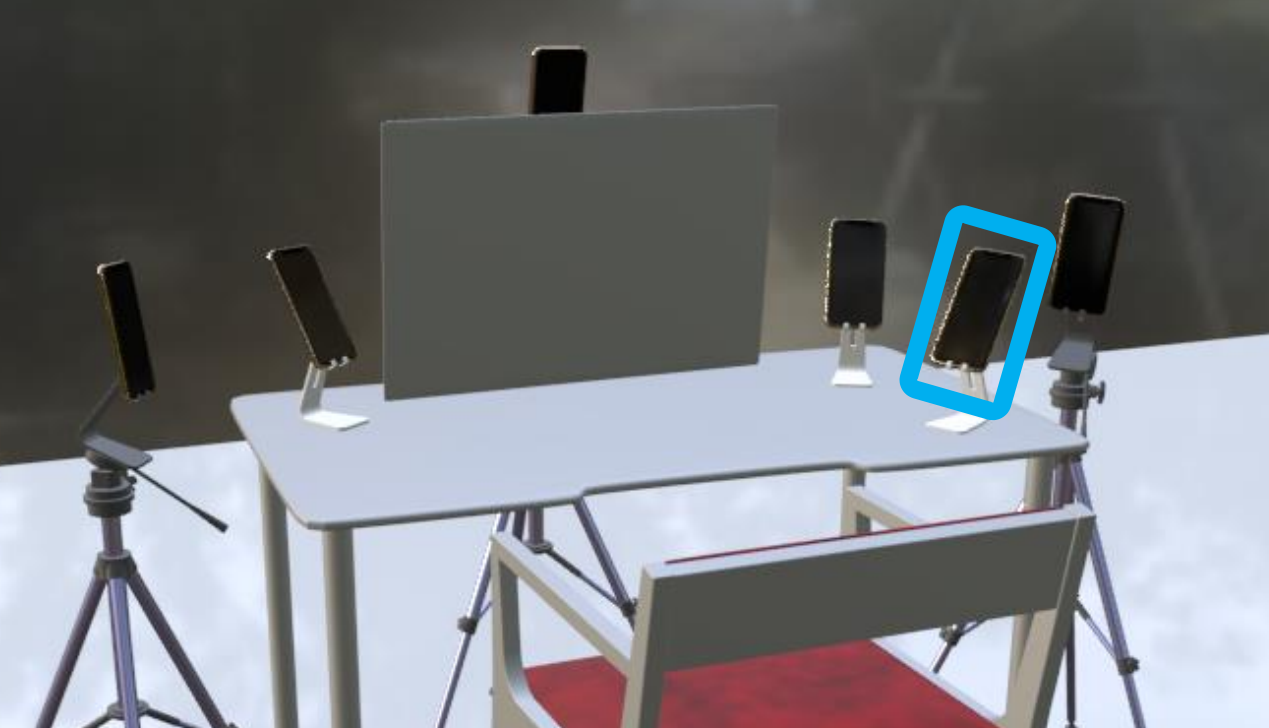
\includegraphics[width=\columnwidth]{scrsht_camera_setup.png}
    \caption{Camera setup for dataset from Hopkins university}
    \label{fig:Hopkins-camera-setup}
\end{figure}


We need additional data to create and validate our technique for analysis. We'll extend the methodology from \cite{zappella} and use the same dataset as in this paper. This dataset is the JHU-ISI Gesture and Skill Assessment Working Set (JIGSAWS), a dataset composed of videos of surgical operations. They use linear dynamical systems to classify the activity present in each segments of the videos. We investigate possible improvements and adapt from classification to tic detection. Dynamical systems are made of two components, one for the structure of the signal, the projection, and one for the dynamics, the transition matrix. In standard methods, the learning of the projection is done independently from the dynamic's learning. But the goal of the projection is to find a latent space where the dynamics of the signal is linear and which is appropriate for the task we want to achieve later in the pipeline. Both objectives of the projection can benefit from a joint learning of the model's parameters. Therefore we investigate how learning them jointly can help the later detection or classification algorithm. We also explore how non-linear dimensionality reduction can help in finding a good latent space for the signal.

As mentioned before, methods from \cite{zappella} are not directly applicable to our task. First, these methods are made for classification purpose, we extend them so that they better fit our detection problem. Secondly, the final goal is to detect the tics on raw videos, this implies we will not have pre-segmented data and thus have to find a way for online detection on frames. Finally, the task is a binary classification problem but the \textit{non-tic} behavior is not a behavior per se, it is the absence of one. This affects the dynamics of the frames and thus the method we should apply when analysing the video.

All the code for this project is on \href{https://github.com/JulesssG/tic-detection}{github}.

%%%%%%%%%%%%%%%%%%%%%%%%%%%%%%%%%%%%%%%%%%%%%%%%%%%%%%%%%%%%%%%%%%%%%%
\section{Dynamical systems for time series modelling}
Dynamical systems are a common approach to time series modelling. For our task, our assumption is that the inherent properties of a segment of the signal are described best by its dynamics. Linear dynamical systems have been shown effective for a variety of task including anomaly detection and activity recognition \cite{zappella, doretto, smoke-detection-LDS}. Dynamical system modelling describe time series using some projection to a latent representation and a matrix describing the evolution of the latent features throughout time. This matrix maps the signal at time $t$ to the signal at times $t+1$.

In our framework, a dynamical system $\mathcal{M}$ has two parameters: a mapping $\bm \Phi_D$ (D is for \textit{decode}) and $\bm A$. $\bm \Phi_D$ define the mapping from the latent representation to the signal space and $\bm A$ is the transition matrix. In practice, we also need $\bm \Phi_E$: the mapping \emph{to} the latent space, i.e. the encoding. So a dynamical system $\mathcal{M} = \big(\bm \Phi_E, \bm \Phi_D, \bm A \big)$ describe a time series with features $y_t \in \mathbb{R}^P$ when:

\begin{equation}
    \begin{cases}
        x_t = \bm \Phi_E(y_t) \\
        y_t = \bm \Phi_D(x_t) \\
        x_{t+1} = \bm A x_t
    \end{cases}
\end{equation}
\noindent In our use case the $\{y_t\}_{t=1}^N$ are the frames of the videos and $\{x_t\}_{t=1}^N$ are the unobserved variable used to discover the dynamics. We reduce the dimension from $P$ to $R$ and so $x_t \in \mathbb{R}^R$.

We can see why the projection used is crucial. If we fix the projection, we can compute $\bm A$ in the least-square sense. Let $\bm X$ is the matrix containing the whole signal represented in the latent space:
\begin{equation*}
    \label{eq:notation+-}
    \begin{gathered}
        \bm X = \begin{pmatrix}x_1 & x_2 & \cdots & x_{N}\end{pmatrix}^T,\ \bm X \in \mathbb{R}^{N \times R}\\
        \bm X_- = \begin{pmatrix}x_1 & x_2 & \cdots & x_{N-1}\end{pmatrix}^T,\ \bm X_- \in \mathbb{R}^{N-1 \times R}\\
        \bm X_+ = \begin{pmatrix}x_2 & x_3 & \cdots & x_{N}\end{pmatrix}^T,\ \bm X_+ \in \mathbb{R}^{N-1 \times R}\\
    \end{gathered}
\end{equation*}
We define $\bm A$ as the transformation from $\bm X_-$ to $\bm X_+$: $\bm X_- \bm A = \bm X_+$. Hence, we have that:
\begin{equation}
    \label{eq:A}
    \bm A = \bm X_-^\dagger \bm X_+
\end{equation}

So if the signal's evolution in the latent space is close to linear, such system will represent the original signal well. Thus segments with different inherent behavior will also have different dynamics, which can be measured using the transition matrix.

The mapping $\bm \Phi_E$ and $\bm \Phi_D$ can be any dimensionality reduction. For these we will use linear projection, a.k.a. the baseline, a fully connected neural network and some convolutional neural networks.

Our baseline comes from \cite{zappella}. In this setup, the projection can be described with a matrix $\bm C = \bm \Phi_D$ and $\bm \Phi_E$ is simply $\bm C^{-1}$. This gives us $\mathcal{M} = \big( \bm C, \bm A)$:

\begin{equation}\refstepcounter{equation}
    \begin{cases}
        y_t = \bm C x_t \\
        x_{t+1} = \bm A x_t
    \end{cases} \tag*{(4)\footnotemark}
\end{equation} \footnotetext{This is a simplified version of classical linear dynamical system. It ignores an additive noise in both equations.}

The projection and dynamics are learned separately and hence given the projection we can compute the transition matrix $\bm A$ using \eqref{eq:A}.

The full signal is represented in the matrix $\bm Y \in \mathbb{R}^{N \times P},\, \bm Y=\begin{pmatrix}y_1 & y_2 & \cdots & y_{N}\end{pmatrix}^T$. For the projection, we'll do a principal component analysis on $\bm Y$ to extract the $R$ components with most variance. Then we project $\bm Y$ onto these principal components and this gives us $\bm X$.

As extension to this method, we use non-linear dimensionality reduction instead of $\bm C$. For this we explore how autoencoders with different architecture are able to discover an appropriate latent space. For the learning, we minimize the reconstruction error the signal. Let $\widehat{Y} = \bm \Phi_D(\bm \Phi_E(Y))$:
\begin{equation}
    \label{eq:loss_rec}
    \mathcal{L}_{rec} = \frac{1}{NP} \norm{\bm Y - \widehat{\bm Y}_{ij}}_F
\end{equation}

Learning the projection and the dynamics jointly give rise to another optimization framework. For it, we use a loss function that uses all variables of the dynamical systems by measuring the reconstruction error of the prediction of the signal:
\begin{equation}
    \label{eq:loss_pred}
    \mathcal{L}_{pred} = \sqrt{\frac{1}{N-1} \sum_{t=2}^{N} \norm{y_t - \bm \Phi_D(\bm A\bm \Phi_E(y_{t-1}))}_2^2}
\end{equation}

Learning both components jointly is a much harder task, so we don't learn all parameters in one go. We initialize the projection and the transition matrix with the computed projection and transition matrix from the separated learning. Then we try to fine tune the parameters using the loss function in \eqref{eq:loss_pred}.

\subsection{Subspace angles and distances between models}
\label{section:subspace-distances}
We have to compare dynamics of video excerpts using their dynamical systems. The dynamical system representation of a signal is not unique, we can apply a change of basis to the matrix $\bm A$ and $\bm C$ that results in the \textit{same} signal representation. Thus we have to use a metric invariant to such transformations. Such metrics are based on the subspace angles between the matrices of dynamical systems.

The computation of the subspace angles assumes a linear projection, so we'll write our dynamical systems as $\mathcal{M}_i = \big( \bm C_i, \bm A_i)$ and whenever the projection is non-linear we set $\bm C=\bm I$. If the models are stable, i.e. $\norm{\bm A_i}_2 < 1$, the subspace angles $\{\theta_i\}_{i=1}^{2N}$ can be computed by solving Sylvester's equations on the matrices $\bm A_i$ and $\bm C_i$. \\
With $\bm P_{ij}$ the solution of:
\begin{gather*}
    \bm P_{ij} = \bm A^T\bm P_{ij} \bm A_j + \bm C_i^T \bm C_j,\ i,j \in \{1,2\}
\end{gather*}

We define $\lambda_i$, $i \in \{1,\dots,2N\}$, as the eigenvalues of $\bm P_{ii}^{-1}\bm P_{ij}\bm P_{jj}^{-1}\bm P_{ji}$, $(i,j) \in \{(1,2),(2,1)\}$. The subspaces angles can then be computed as $\cos^{-1}{(\lambda_i)},\, i\in \{1,\dots,2N\}$

Based on the subspace angles, several distances exist. Two of them are the (squared) Martin and Frobenius distance and are defined as:
\begin{equation}
    d_M^2(\mathcal{M}_i, \mathcal{M}_j) = -\log\prod_{i=1}^{2n}\cos{(\theta_i)}^2
\end{equation}
\begin{equation}
    d_F^2(\mathcal{M}_i, \mathcal{M}_j) = 2\sum_{i=1}^{2n}\sin{(\theta_i)}^2
\end{equation}

This will allow us to directly compare the dynamics of different portion of videos from their dynamical systems.

\subsection{Classification method using the metrics}
\label{section:classification}
For classification, we'll use two different simple yet effective algorithms based on distances: k-Nearest Neighbors (KNN) and Support Vector Machine (SVM) with Radial Basis Function kernel (RBF). Two very popular algorithm that performs well in practice. The kernel function act as a transformation on the distance between points and is defined as:
\begin{equation}
    \mathcal{K}_{RBF}(\mathcal{M}_i, \mathcal{M}_j) = e^{-\gamma d^2(\mathcal{M}_i, \mathcal{M}_j)}
\end{equation}
Where $d^2$ is either the Martin or Frobenius distance and $\gamma$ is a hyperparameter.

%%%%%%%%%%%%%%%%%%%%%%%%%%%%%%%%%%%%%%%%%%%%%%%%%%%%%%%%%%%%%%%%%%%%%%
\section{Experiments}

\subsection{Non-linear dimensionality reduction}

Our first objective is to explore if non-linear dimensionality reduction help us find a suitable latent space for the frames. For this we'll use autoencoders, neural networks with an encoder/decoder structure. Autoencoders are very powerful models for dimensionality reduction, and we can construct arbitrarily complex transformation in the encoding and decoding parts. Each autoencoder's decoder will be the encoder's complement so we'll just describe the encoder's structure from which, it is easy to reconstruct the decoder ($3$d convolutions will become $3$d transpose convolutions, linear layers will becomes linear layers with exchanged input/output sizes, etc.). We design our autoencoder on the basis of several papers such as \cite{temp-regularity-AE, endtoend-AE}.

We'll use three different structures for the encoder: a linear transformation, a one-hidden linear layer with ReLU non-linearity and a temporal convolutional structure also with ReLU non-linearities. Each network will be optimized using the reconstruction error \eqref{eq:loss_rec}. The first one, the \texttt{PCAAE}, serves as a comparison to the PCA model. In PCA, the projection to the latent space is linear, so in theory this network can have equal performance compared to PCA. This, of course, is if we manage to train this network to the global minimum of its loss function. Then the second, the \texttt{OneHAE}, is a fairly simple yet powerful model: a one hidden layer neural network with $200$ hidden neurons. The last category of network, the \texttt{TempConvAE}, uses the signal's structure. By using convolutions instead of simple fully connected layers we can stack more layers, more filters in parallel and it preserves the signal's structure. It is able to preserve the local dependencies between pixels to create appropriate features. We use a temporal convolutional network and vary its depth and number of channels in the hidden layers from $1$ to $5$ and from $4$ to $64$ respectively. This network takes batches of $16$ frames and feed them to $3$d convolutional layers with stride equal to $2$ at the beginning to reduce the dimension of the signal. At the end of the encoder, the signal's dimension will be of order $5000-10000$ per channel for all depths except with only one hidden layer where the signal's order will be higher.

The projection's final objective is not to be able to reconstruct the signal. Hence, a correct evaluation for it in this context would be to use it for a full pipeline: obtaining the dynamical system models induced by it and using this in a real classification or detection task. But such experiments with too many variables are hard to design, run and more importantly results are much less understandable. The capacity to reconstruct the signal will indicate how much information it is able to capture, which is a good starting point. We'll begin by evaluating the models using the reconstruction error on the frame of a video from the team at Hopkins to see if these networks are promising before doing a complete evaluation. This video shows a person with tic disorder standing in a chair, as described in the introduction. We scale the video to $256\times 256$ pixels and it has approximately $30$ FPS. The learning rate of all networks have been optimized and we use Adaptive Moment Estimation (Adam) as optimizer.

We first vary the number of channels and the depth of the convolutional network. We use $10$ seconds of the video. The results are showed in figure \ref{fig:tempconv-channels}.

\begin{figure*}[ht]
    \centering
    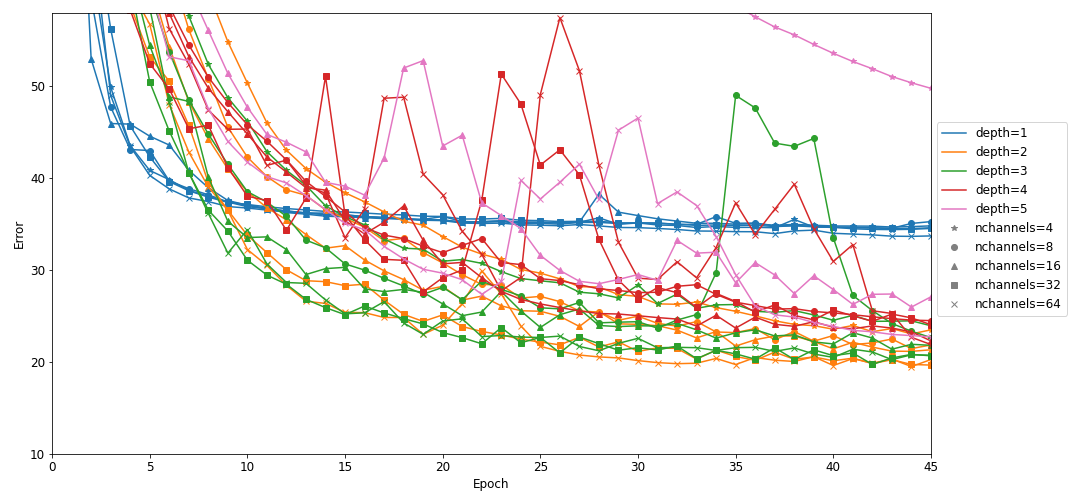
\includegraphics[width=0.7\paperwidth]{reconstruction_error_comparison_tempconv_channels_depth_wrt_epoch.png}
    \caption{Impact of depth and number of channels for temporal convolutional network on the reconstruction error}
    \label{fig:tempconv-channels}
\end{figure*}

In terms of reconstruction error it seems like adding more than two layers doesn't induce a significant improvement. However, it increases the variance during training and computational needs. Increasing the number of channels also reduce the error but it quickly saturate. The network with $2$ hidden layers and $32$ channels for all layers seems like the sweet spot, we'll use this particular architecture for the next experiments. To compare this network to other dimensionality reduction models we have to map the signal to the same number of dimension. So next, we measure how enforcing the number of dimensions to a fixed number affect the network's power. Again, we use $10$ seconds of a $256\times 256$ video and the measure is the reconstruction error presented in \eqref{eq:loss_rec}. This is shown on figure \ref{fig:latent-dimension}.

\begin{figure}[h]
    \centering
    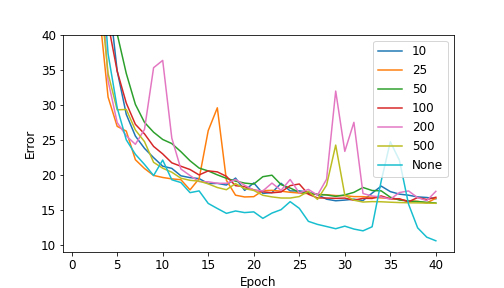
\includegraphics[width=\columnwidth]{latent_dimension_comparison_tempconv.png}
    \caption{Effect on reconstruction when enforcing the latent dimension. Numbers in the legend correspond to the dimension in the latent space.}
    \label{fig:latent-dimension}
\end{figure}

As we can see, the problem with this approach is that the mapping to enforce the dimension in the latent space is linear. This network's goal is to learn time-dependent non-linear feature. At the end of the encoder, the signal is still in very high-dimension so reducing drastically the signal with a linear projection hurts the network's power badly. But mapping to $10$ or to $500$ dimensions doesn't affect the power in a significant way. That would be an argument towards deeper architecture. So that at the end of the non-linear layer, the signal's size is as needed.

We now compare all dimensionality reduction models by showing their respective reconstruction error during training. We use the same video as before, but increase the duration of it to $30$ seconds. For the temporal convolutional network, we show the curve of it with and without a linear projection enforcing the dimensionality of its latent space. Except for the convolutional model without linear mapping, all models project the signal onto $\mathbb{R}^{10}$. This is shown in figure \ref{fig:rec-error-all-models}.

\begin{figure}[h]
    \centering
    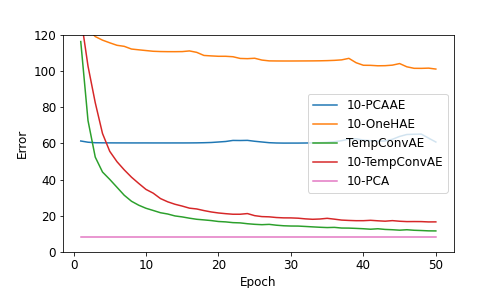
\includegraphics[width=\columnwidth]{figures/reconstruction_error_comparison_pca_oneh_tempconv.png}
    \caption{Reconstruction error for all dimensionality reduction models}
    \label{fig:rec-error-all-models}
\end{figure}

Even without enforcing the dimension, the convolutional layer does not outperform the original PCA model. The two other models are clearly worse than PCA and the convolutional models. From these results, we choose not to continue into this non-linear dimensionality reduction technique for the projection of dynamical systems. It is likely that such networks can find better projection for our task, but for this it may be better to use a network known to be effective for video compression, like U-Net \cite{ronneberger2015unet}, or other video compression algorithms. We prefer to focus on discovering how learning the projection and the transition matrix jointly can help us and extend the techniques to tic detection.

\subsection{Activity recognition on JIGSAWS dataset}
We test our methods by classifying an existing dataset: the JHU-ISI Gesture and Skill Assessment Working Set (JIGSAWS). This dataset is composed of videos of surgical operations done by surgeons using robotic hands. These operations, or task, are: knot tying, needle passing and suturing. For each of these task we have seven or height surgeons performing the task multiple times. There is two captures for each trial, filming from slightly different angles. Each task can be decomposed in atomic surgemes: \textit{Positioning needle}, \textit{Reaching for needle with right hand}, \textit{Orienting needle} etc. For a complete description of the dataset, refer to \href{https://cs.jhu.edu/~los/jigsaws/dwnld/JIGSAWS.pdf}{this link}. These surgemes, or gestures, will be the activities we will detect. Each video has information on what activity is happening at every frame, which gives us a decomposition of the video for our activity recognition. In total for each task, there is between $1$ and $2.5$ hours of videos at $30$ FPS and, as before, we scale each video to $256\times 256$ pixels.

\subsubsection{Classification using pre-segmented data}
\label{section:classification-presegmented}

First we'll classify the fragments from the pre-segmented videos according to their inherent activities using the supervised classification algorithm described in \ref{section:classification}. We use PCA to project the signal onto $\mathbb{R}^R$ and try both separated learning and separated learning with joint fine-tuning. The former uses equation \eqref{eq:A} to compute the transition matrix and the latter optimize further the other model's parameters using \eqref{eq:loss_pred}. For this experiment and the followings we fix $R=10$. We use the same subspace for all experiments to be consistent and choose this number of dimensions because each principal component starting from the eleventh explain $1\%$ or less of variance in the frames for both the JIGSAWS dataset and the videos from Hopkins university. It results in a projection explaining $75\% -80\%$ of the variance while having only $\frac{P}{R}\approx \frac{1}{6554}$ of the original number of dimensions. That allow us to highly reduce the signal's dimension while keeping enough variance of the original to analyze it. This experiments has two main objectives: confirm that the methods can detect an activity on raw video data and check whether the joint fine-tuning of the projection and the dynamic matrix helps the classification algorithm.

For the baseline approach, we classify fragments from all surgeons separately using $5$-fold cross-validation and average the accuracy across them and within the tasks. That gives us a single measure per task and algorithm. We use raw accuracy and weighted accuracy, both measures are averaged across splits. We show the average weighted accuracy as the gestures are not evenly distributed and so the raw accuracy is not a representative measure for underrepresented gestures as it will most likely overclassify the dominant gestures.

\begin{figure*}[t]
    \centering
    \begin{subfigure}{0.25\paperwidth}
      \centering
      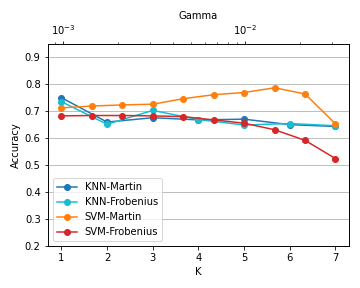
\includegraphics[width=0.25\paperwidth]{evaluation_jigsaws_accuracy_baseline_Knot_Tying.png}
    \end{subfigure}%
    \begin{subfigure}{0.25\paperwidth}
      \centering
      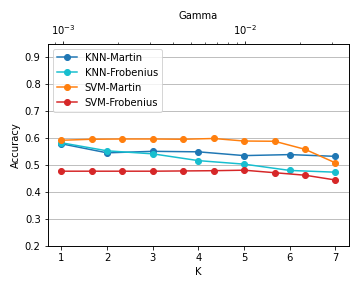
\includegraphics[width=0.25\paperwidth]{evaluation_jigsaws_accuracy_baseline_Needle_Passing.png}
    \end{subfigure}%
    \begin{subfigure}{0.25\paperwidth}
      \centering
      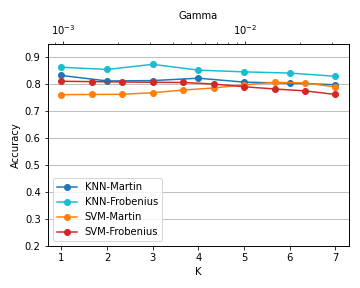
\includegraphics[width=0.25\paperwidth]{evaluation_jigsaws_accuracy_baseline_Suturing.png}
     \end{subfigure}
     \begin{subfigure}{0.25\paperwidth}
      \centering
      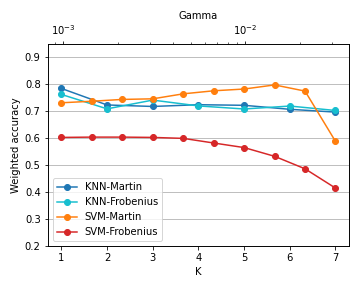
\includegraphics[width=0.25\paperwidth]{evaluation_jigsaws_weighted_accuracy_baseline_Knot_Tying.png}
    \end{subfigure}%
    \begin{subfigure}{0.25\paperwidth}
      \centering
      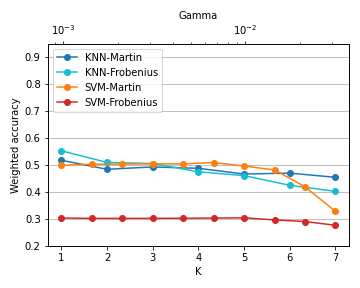
\includegraphics[width=0.25\paperwidth]{evaluation_jigsaws_weighted_accuracy_baseline_Needle_Passing.png}
    \end{subfigure}%
    \begin{subfigure}{0.25\paperwidth}
      \centering
      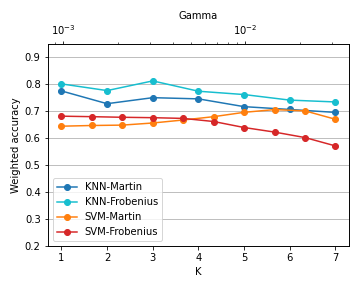
\includegraphics[width=0.25\paperwidth]{evaluation_jigsaws_weighted_accuracy_baseline_Suturing.png}
     \end{subfigure}
    \caption{Average classification accuracy for all subjects on JIGSAWS dataset. Each colun corresponds to a task. From left to right: \textit{knot tying}, \textit{needle passing} and \textit{suturing}.}
    \label{fig:eval-jigsaws-accuracy-baseline}
\end{figure*}

Results are shown on figure \ref{fig:eval-jigsaws-accuracy-baseline}. From the plots, we can tell that it is harder to classify activities in the \textit{needle passing} task. In the other activities, the accuracy is acceptable given the simplicity of the pipeline. The number of activities present in each task is $6$, $10$ and $10$ for \textit{knot tying}, \textit{needle passing} and \textit{suturing} respectively. It becomes $6$, $8$ and $9$ as we remove activities that are not represented enough. Activities removed appears up to $6$ times, which is tiny compared to other gestures appearing more than $100$ times in average. Even if the \textit{suturing} task has the highest number of gestures, best classification results and highest stability is obtained in it. We can deduce that it is the easiest task to classify. The Frobenius distance couples well with the k-Nearest Neighbors classifier but doesn't perform well with Support Vector Machines. The Martin distance seems more stable accross algorithms. Overall, results shows that the baseline can indeed recognize activities in pre-segmented videos.

Early results indicated that the joint learning approach results were not significantly better than the baseline. As it involves hyperparameter tuning and optimization for every fragment it is computationally intensive and for the sake of time we don't use the whole dataset for it. Instead, we use only one task and one surgeon which gives us around $20$ minutes of video. As for the baseline, we use $5$-fold cross-validation to compute the average accuracy obtained across splits. We fine-tune the parameters of each fragment for $15$ epochs using a globally optimized learning rate.

\begin{figure}[h]
    \centering
    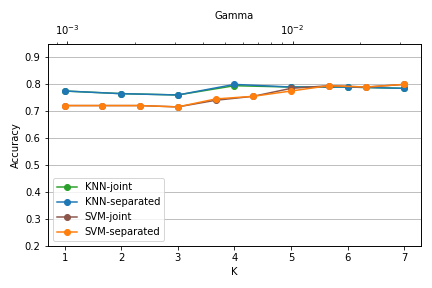
\includegraphics[width=\columnwidth]{evaluation_jigsaws_accuracy_joint_vs_separated.png}
    \caption{Comparison of accuracy between separated learning with or without fine-tuning on suturing task, surgeon \textit{B}}
    \label{fig:eval-jigsaws-joint-vs-separated}
\end{figure}

As we can see in figure \ref{fig:eval-jigsaws-joint-vs-separated}, the fine-tuned model perform as the baseline. That, in fact, is not surprising when looking at the hyperparameter, i.e. the learning rate, tuning and the evolution of the loss during training. After the initialization using the parameters from separated learning, the learning rate we use to minimize the loss function is $5\cdot10^{-7}$. When taking a higher learning rate, the loss function worsen as we optimize. And even with such low learning rate, some fragments still suffer from a small increase in their objective value. Their is low probability that each models ends up at a local minima when using the baseline, which indicates that learning both models separately is close to optimal.

\subsubsection{Comparison of prediction error between models}
\label{section:pred-error}
As previously mentioned, the classification techniques in \ref{section:classification-presegmented} are not directly applicable for several reasons. In anomaly detection the videos are not pre-segmented. In fact in the end, the goal is to develop an online tic detection framework. Hence, we explore a potential online detection algorithm based on the reconstruction error of the frames' prediction \eqref{eq:loss_pred} of linear dynamical systems.

First, we pick a particular video and a particular gesture. For all occurrences of the gesture in the video, we create a model using the baseline approach. Then for every model we compute the prediction's reconstruction error of all frames to see how they behaves through the video. We expect that the reconstruction errors go down for each model's own fragment and hope that the error of a model go also down when in another fragment of the same gesture. If that is the case, that would mean that the models generalize for other fragments of same gesture and thus that we could train an online classifier on a video using pre-fitted models, just using these errors as features.

From now on, we will focus our analysis on the \textit{suturing} task and the Martin distance. As they seem to be the most stable choice. Results are shown in figure \ref{fig:pred-error-jigsaws}. There is two curves per color, the horizontal curve (at $y=0$) is a mask showing the occurrence of the gesture for the model of the same color and the other is the error.

\begin{figure}[h]
    \centering
    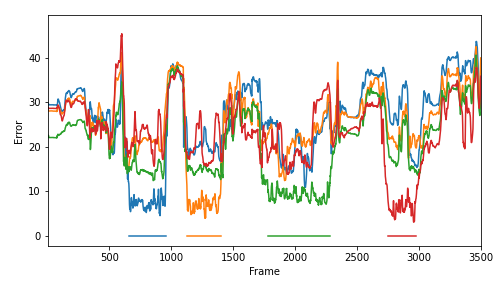
\includegraphics[width=\columnwidth]{prediction_error_models_jigsaws_Suturing_B_trial1_g3.png}
    \caption{Reconstruction error of prediction for models created with different occurrences of gesture \textit{Pushing needle through tissue}}
    \label{fig:pred-error-jigsaws}
\end{figure}

We can see that the reconstruction of different models are quite related, but not enough to easily build a classifier upon. We tried to build a classifier on top of these errors by using Support vector Machine with RBF kernel and optimizing both the $\gamma$ and the regularization parameter with grid search. We try two different setup. In the first one, we create the models and detect the gesture on the same video. Models used for training are all models but the first occurrence's model and we train the algorithm with (errors ,label) tuple for all frames from the end of the first occurrence. To test, we feed the errors for all frames and try to detect the occurrence of the missing model. In the second setup, we use two videos. We use the entire first video for training, and the second for testing. To test we compute the reconstruction error of all models from the first video on all frames of the second and feed it to the classifier trained on the first video.

Results are not very conclusive. In the first setup the algorithm detect no other fragment with the same gesture and in the second setup the reconstruction errors are too noisy to detect the gesture presence. Even when using the same video but with a different capture, so we only modify the angles from where it is filmed, the classifier's performance is poor. If the models generalized better on other videos, we could train using the reconstruction error on videos were the models do not originate from, and that should yield a much more sensible algorithm.

So the difficulty to train a classifier from the reconstruction error comes from the fact that the models have difficulties capturing the dynamics of other occurrences of the same gesture and the fact that the reconstruction error is noisy. To help the first issue, it may help to cluster models of the same gesture together so that their Martin distance is low. To achieve this, an example strategy would be to fix all projection matrices and optimize all transition matrices of a same activity using a loss combining the reconstruction error of the prediction and the intra-cluster distance. So for a particular activity and $k$ models belonging to it $\big \{\mathcal{M}_i \big \}_{i=1}^k$, assuming that each model's projection is linear we optimize their transition matrix by minimizing:

\begin{equation}
\begin{split}
    \label{eq:clusterloss1}
        \mathcal{L}_{cluster} = & \alpha \sum_{i}\norm{\bm X_+^i - \bm A_i X_-^i}_F^2  \\
                            & + (1-\alpha)\sum_{i\neq j}d_M^2(\mathcal{M}_i, \mathcal{M}_j)
\end{split}
\end{equation}

Where $\alpha \in [0,1]$ is a hyperparameter and the notation $X_-^i$ or $X_+^i$ is defined as in \eqref{eq:notation+-} with the superscript specifying the particular set of frames. We tried such approach but to be able to minimize this loss we have to compute the derivative of the Martin distance. This computation is based on solutions to matrix equations, it is possible that we did not manage to minimize the Martin distance because our solutions were inexact, but in any case this computation is not trivial. If we were able to cluster the models together, chances are that it will improve the generalization power of the models within the same activity. In the evaluation of this framework, given a set of frames, we would minimize the induced model's transition matrix with this loss for all activity and the activity were this loss is the lowest is the activity that matches best the frames. Hence, we guess this is the activity present in this portion of video.

The second issue could be mitigated by aggregating the reconstruction error of multiple frames to do the classification. The errors are noisy on a frame basis but looking at a batch of frames can help stabilize the classification and have more continuous portion of video containing the same activity.

\subsubsection{Comparison of the Martin distance}
It is difficult to create models with low reconstruction errors on other model's gesture occurrence. The reconstruction error depends on the exact transformation induced by the projection and the transition which makes it very sensitive to any change in the frames. But measures described in \ref{section:subspace-distances} are more robust to such transformations. They are more sensible to serve as basis for a classifier.

Using the same video and gesture as for the reconstruction error, we'll measure the Martin distance between the models based on this gesture and a model fitted in a moving window fashion. We use a typical length for the gesture's occurrence as number of frames used for the moving window model. Namely, we pick the median of all occurrences of this gesture in this video. Contrary to the mean, this will be robust to a gesture's occurrence with significantly smaller length for example. Then, we plot the distances between all models and the moving window models computed on all frames. This is shown in figure \ref{fig:martin-distance}.

\begin{figure}[h]
    \centering
    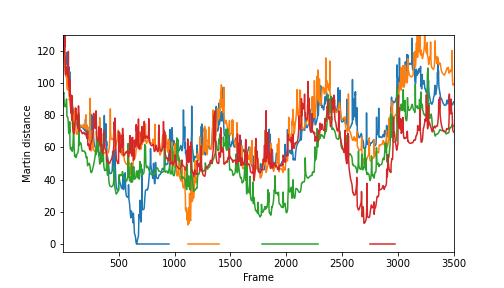
\includegraphics[width=\columnwidth]{martin_distance_jigsaws_Suturing_B_trial1.png}
    \caption{Martin distance between model of gesture \textit{Pushing needle through tissue} occurrences and moving window model, on a particular suturing video of JIGSAWS dataset}
    \label{fig:martin-distance}
\end{figure}

We see that the distance drops when the gesture occurs. From this distance, we can thus detect the gesture. The problem here is that the method is not applicable in a test setting as is. It has the same problem has the method in last section, to be usable it must generalize for other videos. From what we observed, this was not the case.

From here, two directions are possible. It is possible that by aggregating the Martin distance between a lot of models and a moving window model, i.e. increasing the number of feature, would yield enough information to detect activities. Then as the number of models in the dataset grows, the probability to have a model that matches will grow and thus the algorithm will improve. A problem with this approach is that it is computationally intensive as the subspace angles calculation needed for the distances is based on solutions of matrix equations. For the other direction, instead of using more data we could try to fit better models. As in the last section, we could minimizing the Martin distance between all models of the same activity. Then in a similar manner, given a set of frame, we can minimize the Martin distance of the model produced by these frames and the models of each activity. In the end the activity with smallest distance between its cluster and the model is the detected activity.

\begin{figure*}[ht]
    \centering
    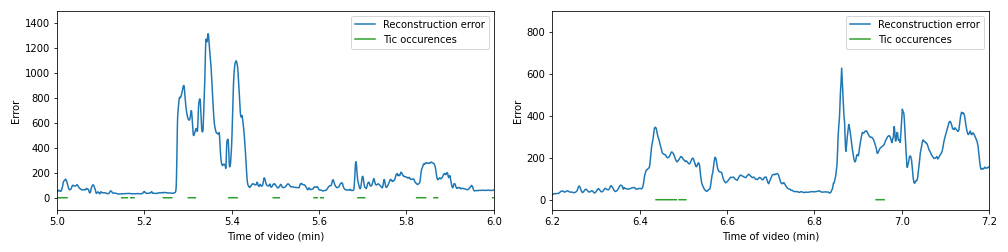
\includegraphics[width=0.8\paperwidth]{tic_detection_pred_error_V12.png}
    \caption{Reconstruction error of prediction for a portion of one video of subject with tic disorder}
    \label{fig:tic-detection-pred-error}
\end{figure*}

\subsection{Tic detection on Hopkins dataset}
We move now to the dataset created by the teams at John Hopkins university. The dataset contains $3$ video of $15$ minutes. Each video contains the same subject, engaged in a high tic activity.

The subject on the video has particularly subtle tics. The majority of them are hard to see with the naked eye even if paying close attention. That will make the detection very hard and it is important to keep this is mind when looking at the results. The subject's tics consist in either moving the nose or the eyebrows. It is not hard to guess how hard that can be to detect such change in the frames with techniques that are based on the general dynamics of the video.

\subsubsection{Classification using pre-segmented data}
We first try the same classification methodology than for the JIGSAWS dataset. We use cross-validation with $5$ splits on each video to compute the average accuracy across splits. We use KNN with $K\in \{1,\dots,7\}$ and SVM optimizing $\gamma$ in a logarithmic space from $2^{-7}$ to $2^{-5}$. Sadly, the algorithm is not able to detect any tics as its performance is not better than random guessing, which clearly indicates that the method does not work for this data.

\subsubsection{Reconstruction error}
To be able to visualize how our method behaves, we try another approach. We fit a linear dynamical system using all frames labelled as normal. Then we plot the reconstruction error of the prediction, again using formula \eqref{eq:loss_pred}, to see if the prediction of the model is worse for fragments labelled as tics. As the video is long, instead of fitting the PCA model to all normal frames, we randomly select one quarter of the normal frames. We show this curve for a portion of two videos on figure \ref{fig:tic-detection-pred-error}.

In addition to being hard to see, tics are very short. Short tics would only have significantly different dynamics if they were abrupt which they are not. The plot on the right shows a section were the reconstruction error and the tic occurrence correlate pretty well. It is not sufficient to conclude anything as taking this as an example is cherry picking but it gives us hope that with more visible tics and more work in the creation of the models, the technique can indeed detect tics.

%%%%%%%%%%%%%%%%%%%%%%%%%%%%%%%%%%%%%%%%%%%%%%%%%%%%%%%%%%%%%%%%%%%%%%
\section{Conclusion}
In conclusion, while the extensions of the activity recognition techniques to tic detection have not proven to be effective yet, there is a lot of potential for improvement. The minimization of the Martin distance can be a key element to improve the overall algorithms capacity. Not only could it produce clustered models but it would also allow to incorporate the final detection or classification decision into a loss function. This could make the joint fine-tuning of dynamical systems significantly better.
%%%%%%%%%%%%%%%%%%%%%%%%%%%%%%%%%%%%%%%%%%%%%%%%%%%%%%%%%%%%%%%%%%%%%%
\bibliographystyle{unsrt}
\bibliography{bibliography}
\end{document}
